\documentclass{article}

\usepackage{amsmath}
\usepackage{graphicx}
\usepackage{hyperref}
\usepackage[utf8]{inputenc}
\usepackage{minted}

\title{Vampire Survivor game}

\author{Christian Linde Ahrnkiel\\
Odense Tekniske Gymnasium
}

\date{28. feburar 2025}

\begin{document}

\maketitle
\tableofcontents

\section{Indledning}
    \subsection{Formål}
    Formålet med dette projekt er at lave et spil, som er inspireret af spillet "Vampire Survivors". 
    Spillet er et 2D top-down-view spil, hvor målet er at overleve så længe som muligt, 
    mens der kommer fjender som man skal bekæmpe. På figur \ref{fig:vps} kan man se et billede af spillet.

    \begin{figure}[h]
    \centering
    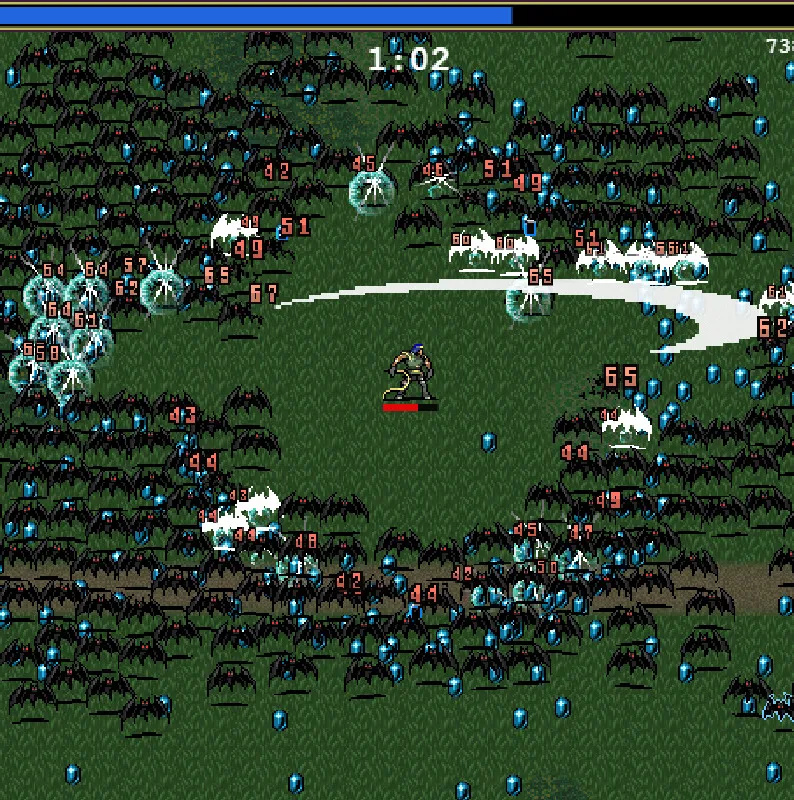
\includegraphics[width=0.5\linewidth]{vps.png}
    \caption{\label{fig:vps}Billede af spillet Vampire Survivors.}
    \end{figure}

    I dette projekt har jeg lavet en simpel version af spillet, i python med biblioteket pygame.
    Man kan se den endelige version af spillet på figur \ref{fig:game}.

    \begin{figure}[h]
    \centering
    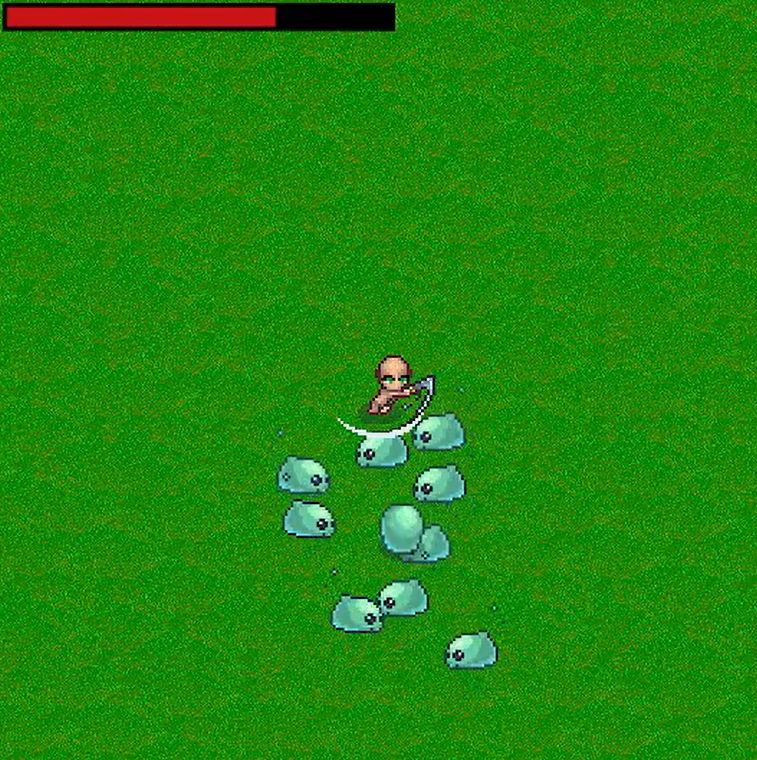
\includegraphics[width=0.5\linewidth]{game.png}
    \caption{\label{fig:game}Billede af spillet jeg har lavet.}
    \end{figure}

\section{Spiller bevægelse}
    \subsection{Bevægelses system}
    For at kunne ungå fjenderne, skal spilleren have en måde at kunne bevæge sig rundt.
    Normalt i spil får man spilleren til at bevæge sig rundt og får et kamera til at følge efter spilleren. 
    Hvor kameraet et det vi ser. Men i pygame er der ikke sådan en funktion. Så det der vil ske er at spilleren vil bare løbe ud af skærmen.
    For at løse dette problem, har jeg lavet spillet sådan at spilleren er altid i midten af skærmen, og at baggrunden og fjernderne bevæger sig i stedet for spilleren.
    Det har jeg gjort ved at have en variabel som hedder "speed", og den trækker jeg fra, eller lægger til, 
    baggrundens og alle fjerndernes x eller y koordinater, afhængig af hvilken retning spilleren bevæger sig.
    Det kan man se her:

    \begin{minted}{python}
    if keys[pg.K_w]:
        grass_y += speed
        player_moving = "w"
        for s in slimes:
            s.y += speed
     if keys[pg.K_s]:
        grass_y -= speed
        player_moving = "s"
        for s in slimes:
            s.y -= speed
    if keys[pg.K_a]:
        grass_x += speed
        player_moving = "a"
        for s in slimes:
            s.x += speed
    if keys[pg.K_d]:
        grass_x -= speed
        player_moving = "d"
        for s in slimes:
            s.x -= speed
    \end{minted}
    
    Der hvor der står player\_moving = et eller andet, det kommwe jeg ind på senere.

    \subsection{Uendelig verden}
    Men nu er der et andet problem. Når spilleren bliver ved med at bevæger i den samme retning,
    ender spilleren med at løbe ud til kanten af baggrunden, da baggrunden er det billede og ikke en uendelig verden.
    For at løse dette problem, tegner jeg baggrunden 9 gange, og flytter dem i forhold til spillerens position.
    Man kan se det som et gitter, hvor spilleren er i et felt, så bliver felterne rundt om spilleren flyttet fyldt med baggrunden.
    Se figur \ref{fig:gitter} for en visual forklaring. Det røde punkt er spilleren og man kan se bevæger så ned til højre.
    Det blå mærket område er der baggrundene bliver tegnet.

    \begin{figure}[h]
    \centering
    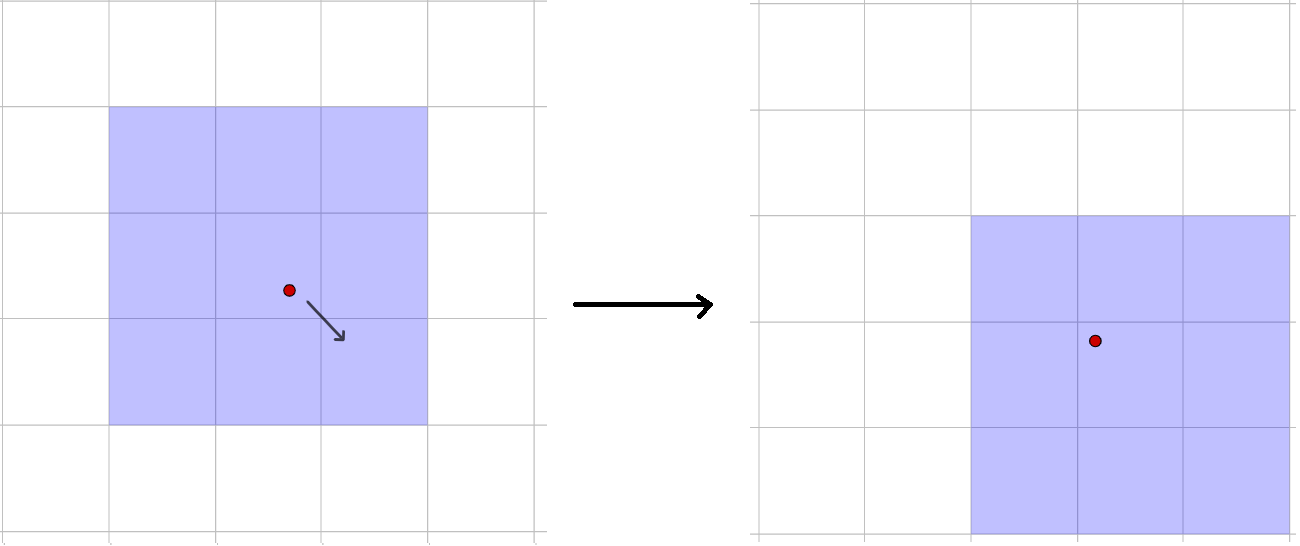
\includegraphics[width=0.75\linewidth]{gitter.png}
    \caption{\label{fig:gitter}Skitse af hvordan baggrunden bliver tegnet.}
    \end{figure}
    
    Koden som gør dette ser sådan ud:

    \begin{minted}{python}
    for x in range(-1,1):
        for y in range(-1,1):
            temp_gass_x = grass_x%grass_width + grass_width*x
            temp_gass_y = grass_y%grass_height + grass_height*y
            screen.blit(grass_img, (temp_gass_x, temp_gass_y))
    \end{minted}

    Den modulus operatoinen \% til at "simolere" gitteret og til at finde ud af hvor spilleren i forhold til gitteret. 
    
\section{Animationer}
Jeg skal have en spiller og nogle fjender i spillet. Det kraver at jeg har nogle animationer, 
fordi at være en firkant der kæmper imod cirker er ikke så fedt at se på. 

    \subsection{Sprite sheet}
    Så for at have nogle animationer, skal vi bruge nogle sprite sheets. 
    Sprite sheets er et billede med billeder på, som til sammen laver en animation.
    Et sprite sheet kan godt have flere forskellige animationer på. 
    Man bruger sprite sheets fordi at det er hurtigere at loade et billede end flere billeder.
    Man kan se et eksempel på et sprite sheet på figur \ref{fig:sprite_sheet}.

    \begin{figure}[h]
    \centering
    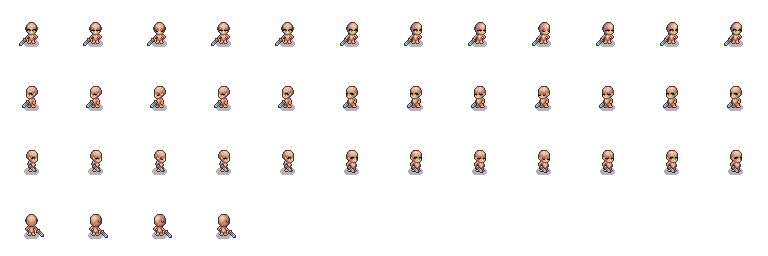
\includegraphics[width=0.75\linewidth]{assets/sprites/Player_Idle.png}
    \caption{\label{fig:sprite_sheet}Sprite sheet af spilleren idle animation.}
    \end{figure}

    Jeg vil vise hvordan jeg indplamenterer spillerens idle animation som et eksempel. 
    Processen er ens for alle animationer. Først åbner jeg billedet med pygame.image.load() funktionen.
    \begin{minted}{python}
    player_idle = pg.image.load("assets/sprites/Player_Idle.png")
    \end{minted}

    Derefter definere jeg spillerens størrelse ud fra billedet. Der er 12 billeder af spilleren på langs, 
    så jeg deler bredden af billedet med 12.
    \begin{minted}{python}
    player_size = player_idle.get_width()//12
    \end{minted}

    Så køre jeg sprite sheetet igennem min load\_sprite\_sheet funktion.
    \begin{minted}{python}
    player_idle_sprites = load_sprite_sheet(player_idle, player_size, player_size)
    \end{minted}

    load\_sprite\_sheet funktionen tager som argumenter, et spite sheet altså et billede, 
    størrelsen af hver sprite i sheetet altså 2 integer.
    Funktionen returnere en liste af alle sprites, som er i sprite sheetet.
    Funktionen ser sådan ud:
    \begin{minted}{python}
    def load_sprite_sheet(sheet, sprite_width, sprite_height):
        sprites = []
        for y in range(0, sheet.get_height(), sprite_height):
            for x in range(0, sheet.get_width(), sprite_width):
                rect = (x, y, sprite_width, sprite_height)
                image = sheet.subsurface(rect)
                image = pg.transform.scale(image, (sprite_width * 3, sprite_height * 3))
                sprites.append(image)
        return sprites
    \end{minted}

    Måden funktionen virker er via subsurface() funktionen. Den tager som argument, en x koordinat, en y koordinat, en bredde og en højde.
    Og så returnere den et nyt billede, som er en del af det originale billede. Det andet det sker i funktionen er bare opsættnings ting subsurface() funktionen.
    Og den skalerer billedet op med 3, fordi at det er for lille.

    Men nu har vi en liste af alle sprites i idle animationen. Men jeg kun have den først række af spritesne, 
    fordi der vinder spilleren mod os. Så jeg laver en ny liste med kun de første 12 sprites,
    ved at køre en for loop igennem de første 12 sprites og tilføje dem til en ny liste.
    \begin{minted}{python}
    player_idle = []
    for i in range(len(player_idle_sprites)//4):
        player_idle.append(player_idle_sprites[i])    
    \end{minted}

    Og så tegne jeg den med blit() funktionen og bruger modulus operatoren til at skifte mellem spritesne.
    Jeg bruger også en variabel som hedder tick, som er hvor mange frames der er gået siden spillet er startet.
    Jeg bruger også et dictionary som jeg kommer ind på senere.
    \begin{minted}{python}
    screen.blit(player_dict_run[player_moving][(tick // 10 % 8)], player_coords)
    \end{minted}

    \subsection{Tilpas animation med retning}
    Så for at finde ud af hvilken retning spilleren bevæger sig, bruger jeg en variabel som hedder player\_moving.
    Den variabel bliver sat til en af de 4 retninger spilleren kan bevæge sig i, når spilleren trykker på enten w, a, s eller d.
    Jeg bruger også et dictionary som hedder player\_dict\_run, som sætter en retning sammen med en liste af billeder til den retning.
    \begin{minted}{python}
    player_dict_run = {
    "w": player_run_w,
    "a": player_run_a,
    "s": player_run_s,
    "d": player_run_d,
    "idle": player_idle
    }
    \end{minted}

    \subsection{Tilpas animation over tiden}
    Når spilleren angreber, skal spilleren have en animation for det. Men der er et problem,
    fordi at det er 4 animationer til når spilleren angreber. En i hver retning. 
    Så for at gøre det, når spilleren angreber, starter en timer. 
    O gså bestemmer jeg hvilken retning spilleren angreber i hvilken retning spilleren bevæger sig i ud fra timeren.
    \begin{minted}{python}
    if event.key == pg.K_SPACE:
        player_attacking = True
    if player_attacking:
        attacktime += 1
    if attacktime >= attackspeed*6:
        player_attacking = False
        attacktime = 0
    \end{minted}

    Resten af punkterne er noget jeg kan komme ind på til den mundlige prøve.
\section{Fjender}
    \subsection{Pathfinding}
    \subsection{Animationer for fjender}

\section{Combat}
    \subsection{Hitbox}
    \subsection{Skade system}
    \subsection{Imune system}
    \subsection{Død system}

\section{GUI}
    \subsection{Health bar}
    \subsection{Død skærm}

\section{Lydeffekter}

\section{Kunklusion}

\end{document}